\section{Evaluation}
\label{Eva}

In this section, we describle our performance evaluation in real-scene
experiments. We distribute 100 TI SensorTag sensors in an about $250~\times~250$
square meters area, with contiki-ng as its operating system. We use different
metrics for various applications and compare our works with other
state-of-the-art works.

\subsection{Routing}
We estimate sensor energy cost by multipling different coefficients on CPU
running time and radio listening and transmitting time and summing them up. The
coefficients are proportional to the working current described in sensor's
DataSheet.
\textbf{Performance}
\begin{figure}[htbp]
	\centering
	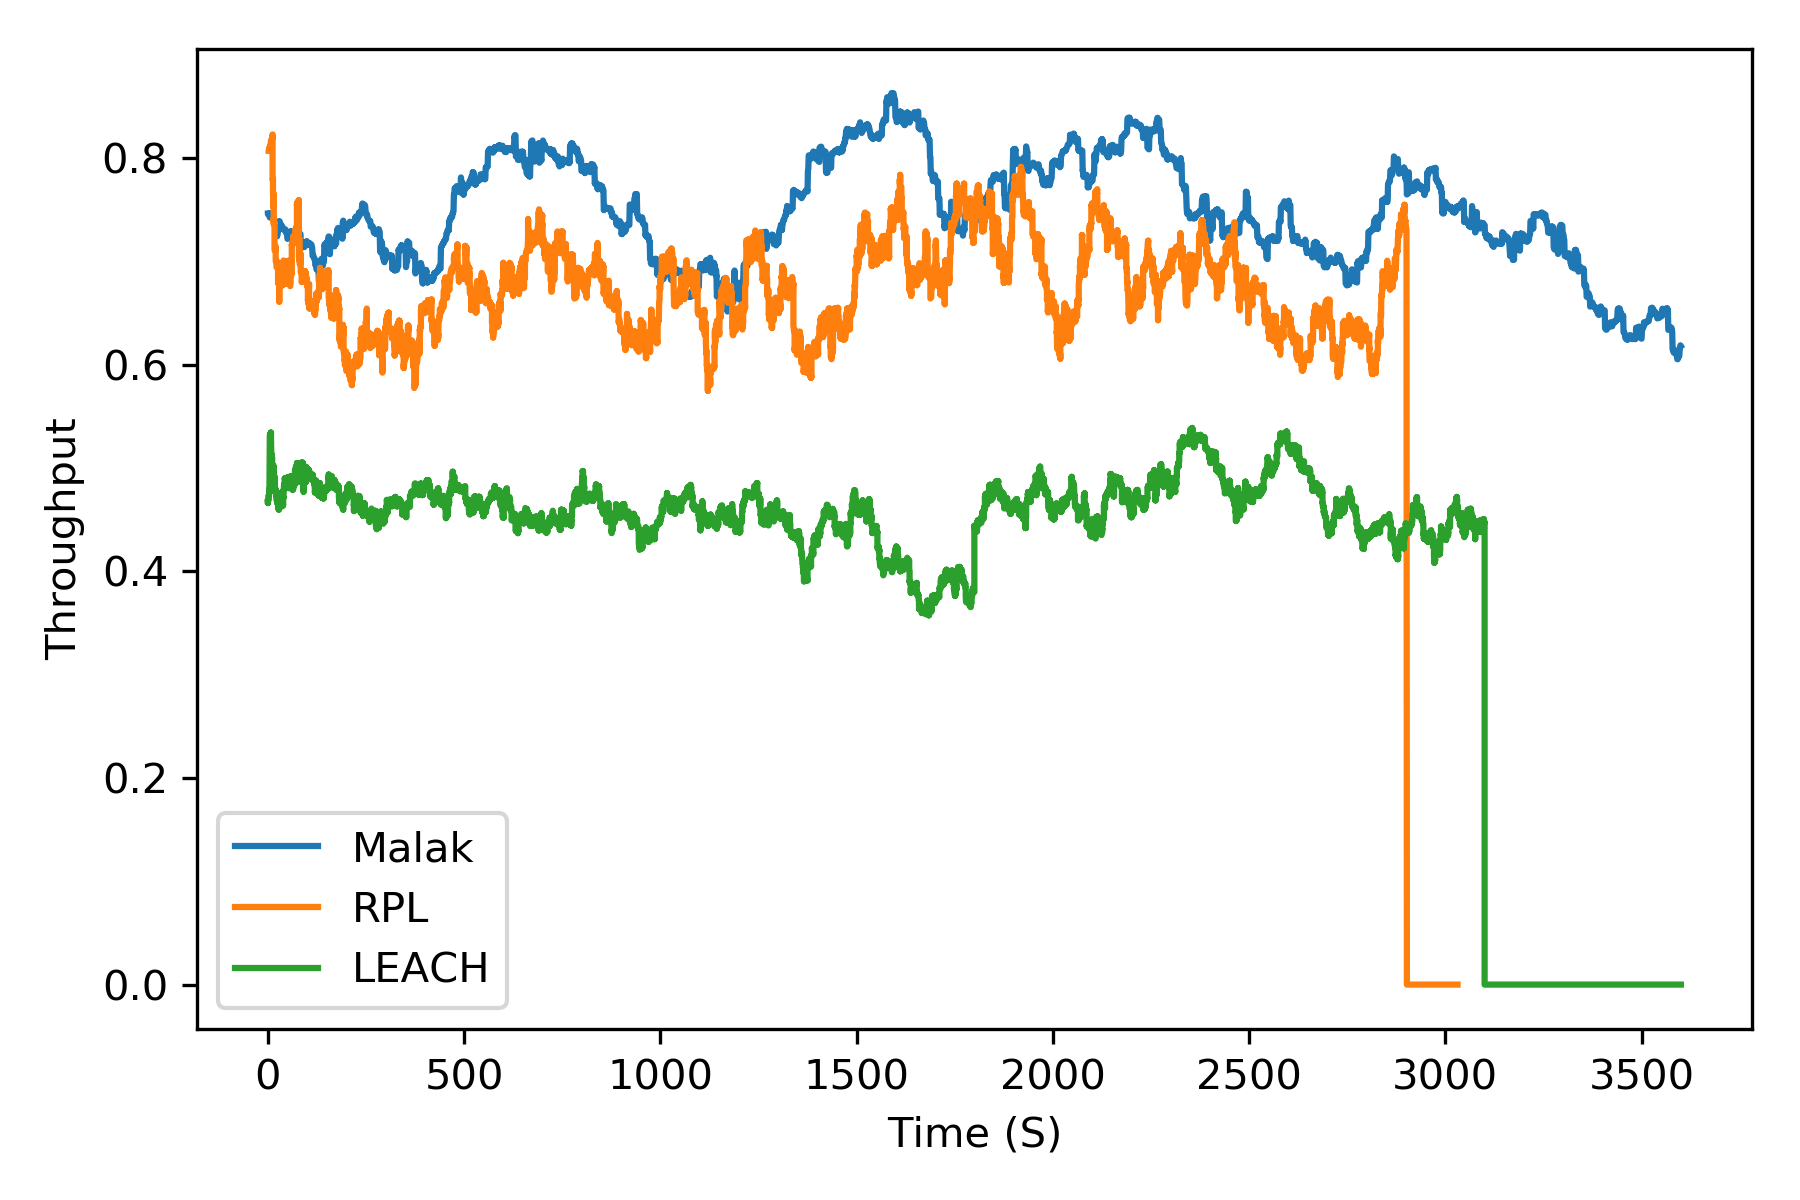
\includegraphics[width=.85\columnwidth]{Figure/throughput}
	\vspace{-0.1in}
	\caption{Routing throughput}
	\label{throughtput}
	\vspace{-0.2in}
\end{figure}
\textbf{Energy efficiency}



\textbf{Fault-tolerance}

\textbf{Scalability}

\subsection{Network Diagnosis}
\textbf{Robustness}

\subsection{AI Node Selection}
\textbf{Scalability}

\subsection{AI Energy Prediction}
\textbf{Prediction accuracy}
\begin{figure}[htbp]
	\centering
	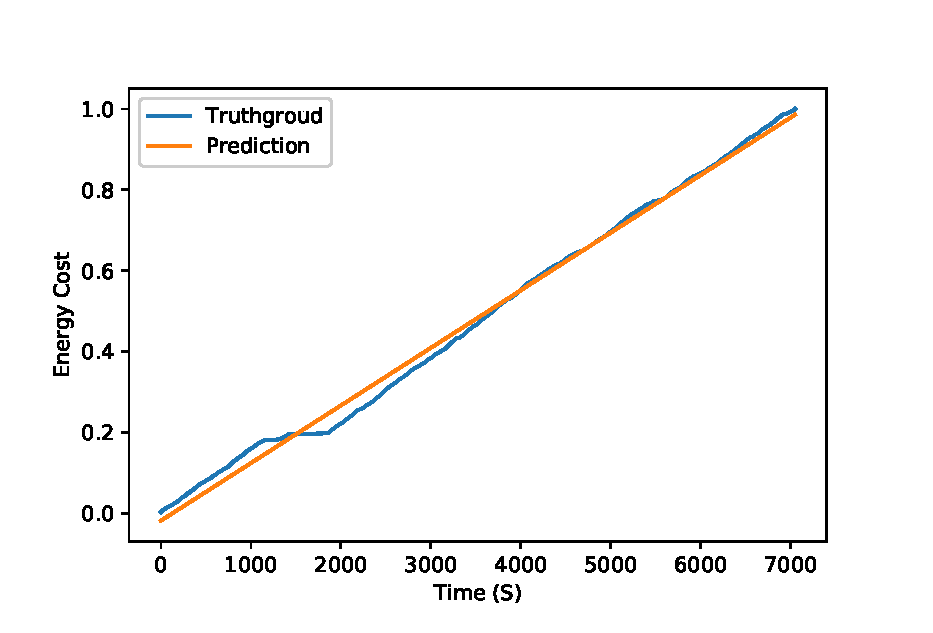
\includegraphics[width=.85\columnwidth]{Figure/energy_pred}
	\vspace{-0.1in}
	\caption{energy prediction}
	\label{energy_pred}
	\vspace{-0.2in}
\end{figure}
\begin{figure}[htbp]
	\centering
	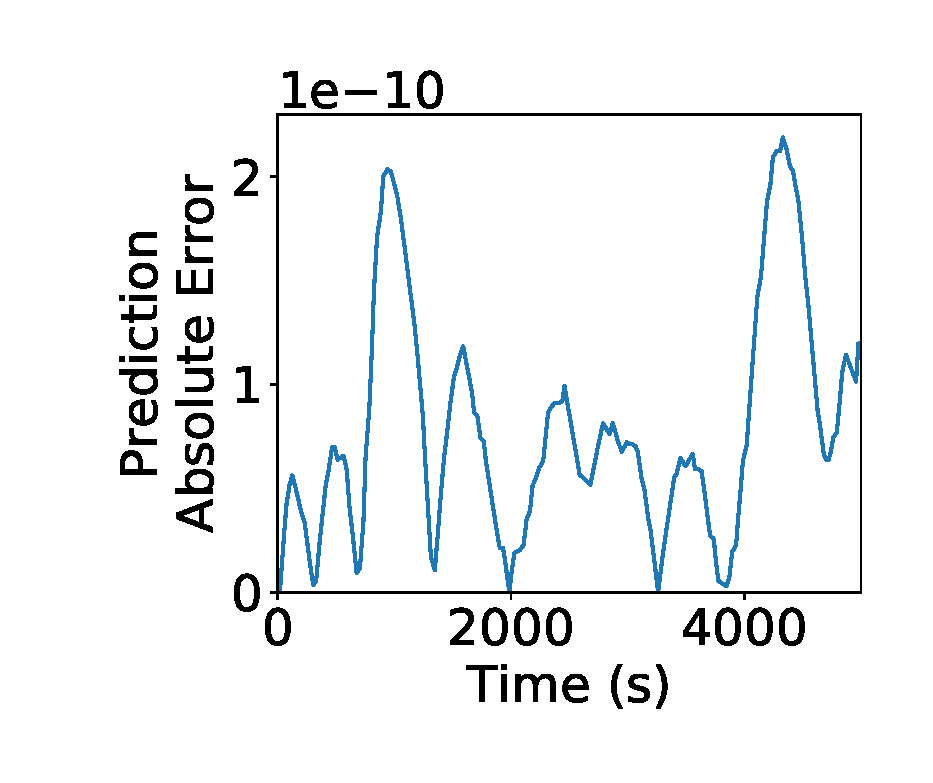
\includegraphics[width=.85\columnwidth]{Figure/energy_pred_err}
	\vspace{-0.1in}
	\caption{energy prediction error}
	\label{energy_pred_err}
	\vspace{-0.2in}
\end{figure}

\subsection{Multi-tasks}
\textbf{Energy Performance}
\textbf{Scalability}


